\documentclass{report}

%%METADATA
\title{International Macroeconomics and Trade }
\author{
Raman Singh Chhina \\ {University of Chicago}
}
\date{}

%%PACKAGES
\usepackage{graphicx}
\usepackage{tabularx}
\usepackage{setspace}
\usepackage{amsmath,amsthm,amssymb}
\usepackage[hyphens]{url}
\usepackage{natbib}
\usepackage[font=normalsize,labelfont=bf]{caption}
\usepackage[margin=1in]{geometry}
\usepackage{hyperref}
\hypersetup{colorlinks=true,urlcolor=blue,citecolor=red}
\usepackage{enumerate}% http://ctan.org/pkg/enumerate %Supports lowercase Roman-letter enumeration
\usepackage{verbatim} %Package with \begin{comment} environment
\usepackage{physics}
\usepackage{tikz}
\usepackage{listings}
\usepackage{upquote}
\usepackage{booktabs} %Package with \toprule and \bottomrule
\usepackage{etoc}     %Package with \localtableofcontents
\usepackage{multicol}
\usepackage{bm}
\usepackage{float}

\definecolor{dkgreen}{rgb}{0,0.6,0}
\definecolor{gray}{rgb}{0.5,0.5,0.5}
\definecolor{mauve}{rgb}{0.58,0,0.82}

\lstset{language=bash,
  frame=tb,
  aboveskip=3mm,
  belowskip=3mm,
  showstringspaces=false,
  columns=flexible,
  basicstyle={\small\ttfamily},
  numbers=none,
  numberstyle=\tiny\color{gray},
  keywordstyle=\color{blue},
  commentstyle=\color{dkgreen},
  stringstyle=\color{mauve},
  breaklines=true,
  breakatwhitespace=false,
  tabsize=3
}
\newtheorem{theorem}{Theorem}
\newtheorem{lemma}[theorem]{Lemma}
\newtheorem{proposition}[theorem]{Proposition}

%%FORMATTING
\onehalfspacing
\numberwithin{equation}{section}
\numberwithin{figure}{section}
\numberwithin{table}{section}
\bibliographystyle{bib/aeanobold-oxford.bst}

%LOGBOOK
\begin{document}

%%LOGBOOK COVER
\maketitle

%TABLE OF CONTENTS
\renewcommand{\thechapter}{\Alph{chapter}}
\setcounter{tocdepth}{1}
\tableofcontents
\etocsettocstyle{}{} % from now on only local tocs

%%LOGBOOK ENTRIES: Introduction
\chapter{\cite{dornbusch1977comparative} Replication}

This document contains the main results from the replication exercise. \underline{ The code is available at the Github repository \href{https://github.com/econ-raman/code_share/tree/main/PS1_DFS}{here}}. 

\section{Equilibrium with no trade costs} \label{solver1}

\ref{fig1} plots the replication of Fig 1 in DFS along with the equilibrium values of $\bar \omega$ and $\bar z$. My results match very closely with those provided in the assignment.

\begin{figure}[H]
  \centering
  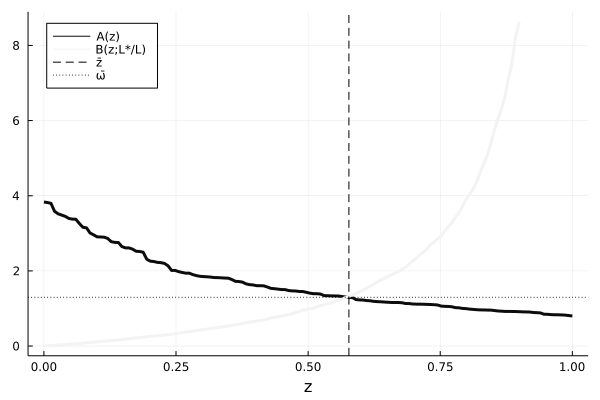
\includegraphics[width = 100mm]{./input/fig1.png}
  \caption{DFS Fig 1. Equilibrium with no trade costs}
  \label{fig1}
\end{figure}

\section{Comparative Statics}

The model solver from \ref{solver1} is used to perform comparative statics in this section. \ref{fig2} plots the $B(z;L^*/L)$ and $B(z;L^{'*}/L)$ where $\frac{L^{'*}}{L^*} = 1.5$. i.e. we check what happens if the foreign country grows by 50\%. The $B(z)$ curve shifts upwards and we get a decrease in $\bar z$ and an increse in $\bar \omega $
\begin{figure}[H]
  \centering
  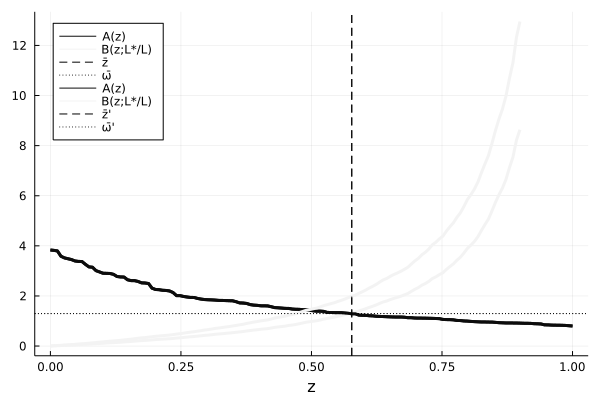
\includegraphics[width = 100mm]{./input/fig2.png}
  \caption{DFS Fig 2. Foreign size increase comparative static}
  \label{fig2}
\end{figure}

Along with the foreign size increase shock \ref{fig2_1} plots the comparative static when foreign undergoes a uniform (20\%) technological progress. This shifts the $A(z)$ curve upwards. And leads to foreign to produce more varieties in equilibrium.
\begin{figure}[H]
  \centering
  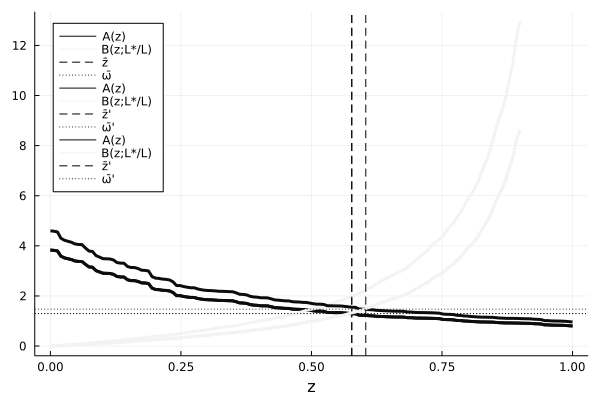
\includegraphics[width = 100mm]{./input/fig2_1.png}
  \caption{Comparative statics for foreign uniform technological improvement and size increase on the same plot}
  \label{fig2_1}
\end{figure}

\section{Equilibrium with trade costs i.e. $g < 1$}

\ref{fig3} plots the replication of Fig 3 in DFS 1977. The model solution for $\bar z$ and $\bar z^*$ is plotted in dashed lines. My results do not exactly match with those provided in the assignement. I suspect this is because of the different solution method. The difference is albeit small.
\begin{figure}[H]
  \centering
  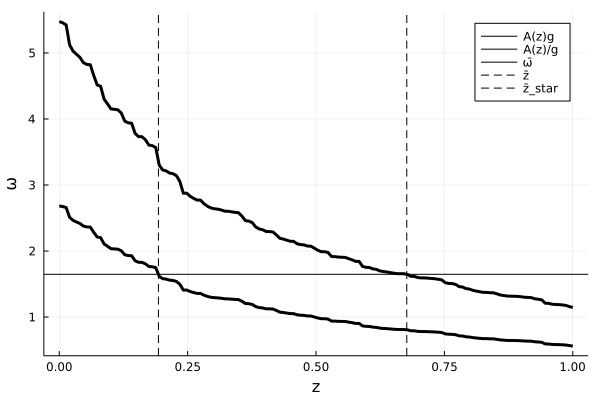
\includegraphics[width = 100mm]{./input/fig3.png}
  \caption{DFS Fig 3. Model solution with general trade costs.}
  \label{fig3}
\end{figure}

\section{Welfare Gains}

An increase in the foreign's productivity leads to an increase in welfare for both the home and foreign. The foreign, however, gains much more. \ref{welfare} plots the gains from trade when foreign goes through a uniform productivity progress ranging 1x to 3x the original level.
\begin{figure}[H]
  \centering
  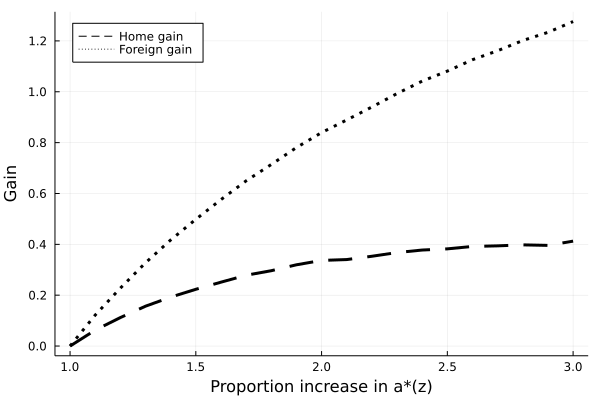
\includegraphics[width = 100mm]{./input/welfare.png}
  \caption{Welfare as a function of increase in foreign's efficiency}
  \label{welfare}
\end{figure}

\section{Gains from trade and volume of trade}

Normalizing the home country's income to 1 in both autarky and in trade, home's welfare in equilibrium is given as
\begin{align}
  \log(1) - \left( \int_0^{\bar z} b(z) \log a(z) dz + \int_{\bar z}^1 b(z) \log(\frac{a^*(z)}{\bar \omega}) dz \right)
\end{align}


and foreign's welfare is

\begin{align}
  \log(\frac{1}{\bar \omega}) - \left( \int_0^{\bar z^*} b(z) \log a(z) dz + \int_{\bar z^*}^1 b(z) \log(\frac{a^*(z)}{\bar \omega}) dz \right)
\end{align}

where $\bar \omega$ is the equilibrium relative wage. The gains from trade as compared to autarky for home is given by
\begin{align}
  \log(1) - \left( \int_0^1 b(z) \log a(z) dz \right)  - \left( \log(1) - \left( \int_0^{\bar z} b(z) \log a(z) dz + \int_{\bar z}^1 b(z) \log(\frac{a^*(z)}{\bar \omega}) dz \right) \right) \\
  \text{Home gains from trade} = \left( \int_0^{\bar z} b(z) \log a(z) dz + \int_{\bar z}^1 b(z) \log(\frac{a^*(z)}{\bar \omega}) dz \right)  - \left( \int_0^1 b(z) \log a(z) dz \right)
\end{align}

Volume of trade in this model is simply the total expenditure of home and foreign countries on their imports. Home spends $\int_{\bar z}^1 b(z) \log(\frac{a^*(z)}{\bar \omega}) dz $ on imports and foreign spends $\int_0^{\bar z^*} b(z) \log a(z) dz $ on imports. So total volume of trade is

\begin{align}
  \text{Volume of trade} =   \int_0^{\bar z^*} b(z) \log a(z) dz  + \int_{\bar z}^1 b(z) \log(\frac{a^*(z)}{\bar \omega}) dz
\end{align}
so,
\begin{align}
  \text{Home gains from trade}  = \text{Volume of trade} - \left( \int_0^1 b(z) \log a(z) dz - \int_{\bar z^*}^{\bar z} b(z) \log a(z) dz  \right)
\end{align}

So, to infer the gains from trade via volume of trade we need to know the autarkic price of the goods which the home is importing and exporting. So, without observing autarkic prices we cannot infer gains from trade just by looking at the volume of trade.

\begin{figure}[H]
  \centering
  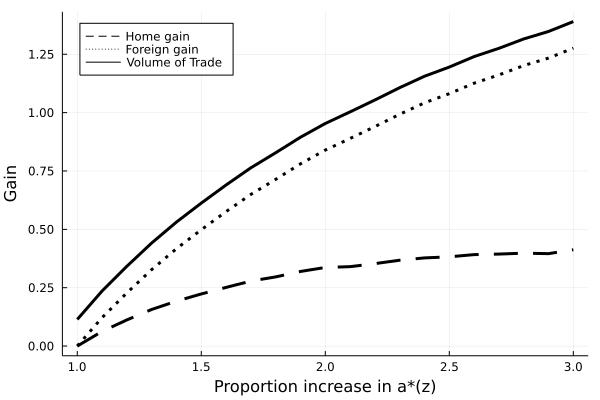
\includegraphics[width = 100mm]{./input/welfare_vot.png}
  \caption{Welfare and VoT with different foreign productivity}
  \label{welfare_vot}
\end{figure}

I am not very sure what the question meant by finding another equilibrium — did you want another set of fundamentals $a$ and $b$ that give the same trade volume but different gains. This is what I understood but didn't implement as it would've had required solving for two two arrays with big dimensions. Rather I use the Fig. \ref{welfare_vot} to show that for a fixed $b$ and a proportional increase in $a^*$ volume of trade and gains move one to one.

%%LOGBOOK BIBLIOGRAPHY
\bibliography{bib/reference.bib}

\end{document}
